\documentclass[11pt]{article}

\usepackage[margin=1in]{geometry}
\usepackage[T1]{fontenc}
\usepackage[utf8]{inputenc}
\usepackage{booktabs}
\usepackage{array}
\usepackage{tabularx}
\usepackage{hyperref}
\usepackage{natbib}
\usepackage{xcolor}
\usepackage{amssymb}
\usepackage{microtype}
\usepackage{graphicx}
\usepackage{lineno}
\usepackage{tikz}
\usetikzlibrary{arrows.meta,positioning,calc}

\definecolor{vfblue}{HTML}{1F4E79}
\definecolor{vfteal}{HTML}{2A7F73}
\definecolor{vflight}{HTML}{EEF5F8}

\hypersetup{
  colorlinks=true,
  linkcolor=vfblue,
  citecolor=vfblue,
  urlcolor=vfblue
}
\setlength{\emergencystretch}{2em}

\title{VariantFlow: a selective-execution engine for efficient population genomic computation on large variant datasets}
\author{
Ehsan Estaji\textsuperscript{1,$\dag$}
\href{https://orcid.org/0009-0005-0838-228X}{\small(ORCID 0009-0005-0838-228X)} \qquad
Jian-Feng Mao\textsuperscript{1,$\dag$}
\href{https://orcid.org/0000-0001-9735-8516}{\small(ORCID 0000-0001-9735-8516)} \\[6pt]
\small \textsuperscript{1}Ume{\aa} Plant Science Centre,
Department of Plant Physiology, Ume{\aa} University,
SE-901\,87 Ume{\aa}, Sweden \\[4pt]
\small \textsuperscript{$\dag$}Correspondence:
       \href{mailto:ehsan.estaji@umu.se}{\texttt{ehsan.estaji@umu.se}},
       \href{mailto:jianfeng.mao@umu.se}{\texttt{jianfeng.mao@umu.se}}
}
\date{}

\begin{document}
\linenumbers
\maketitle
\newpage

\begin{abstract}
\noindent
Population-scale sequencing now produces variant call sets with thousands of
samples and millions of sites, making post-calling analysis a recurring
bottleneck. Because the Variant Call Format stores every field of every record
together, a tool answering a field-limited question still parses the unused
annotations, FORMAT blocks, and per-sample values, which costs time without
changing the result. We present VariantFlow, a command-line engine built on
selective execution, decoding only the fields the current filter, statistic,
or projection requires and preserving original records where possible. On
correctness-matched benchmarks on the 1000 Genomes 3\,202-sample high-coverage
dataset, VariantFlow computed whole-chromosome missingness 8.0--8.5x faster than
VCFtools at a constant 8.6~MB of memory, the chromosome~1 summary taking 128~s
against 1031~s. An index-assisted $\mathtt{FILTER}=\mathtt{PASS}$ predicate ran
123--273x faster than bcftools where block metadata excludes most of the file.
Further gains, reported in Table~1, cover FORMAT-rich filtering on record
subsets, linkage disequilibrium, and export-once Parquet queries served through
DuckDB. Core population-genetic outputs were byte-identical to VCFtools,
per-individual missingness and the site-frequency spectrum matched scikit-allel
exactly, and the missing-data-aware $\pi$ and $d_{XY}$ estimators reproduced
pixy's pairwise counts in every window. By decoding only the fields each
operation requires, VariantFlow brings large-cohort post-calling analysis within
reach of exploratory work on a single workstation. It complements rather than
replaces bcftools, HTSlib, GATK, and VCFtools, and should be of value wherever
large cohort VCFs are repeatedly summarised, filtered, or exported. VariantFlow
is open source (Rust, MIT OR
Apache-2.0) at \url{https://github.com/ehsanestaji/VariantFlow}; version~1.5.0
is archived at
\href{https://doi.org/10.5281/zenodo.21198172}{doi:10.5281/zenodo.21198172}.

\vspace{0.6em}
\noindent\textbf{Keywords:} population genomics, variant call format,
selective execution, missing data, nucleotide diversity, bioinformatics
software, Rust
\end{abstract}
\newpage

\section{Introduction}

The volume of genomic variant data is growing rapidly. Population-scale
sequencing projects now routinely produce Variant Call Format (VCF) files that
describe thousands of samples and millions of variant sites per chromosome
\citep{vcftools}. Once variants have been called, these files are scanned
repeatedly for quality filtering, cohort subsetting, population-genetic
summaries, and conversion to downstream formats. These repeated scans are a
recurring cost in post-calling analysis, and each is typically carried out by a
tool that parses the entire record even when the operation depends on only one or
two of its fields.

This inefficiency follows directly from the VCF design. A VCF record stores
every property of a variant on a single line, beginning with the site-level
fields (position, quality, filter status, and INFO annotations) and continuing,
for every sample in the cohort, with a FORMAT block such as
\texttt{GT:DP:GQ:AD} that encodes the genotype, read depth, genotype quality,
and allelic depths. This layout makes VCF a general exchange format that any
downstream program can read, which is why it has become the standard
representation for variant data. It also means that a program answering a
field-limited question, such as retaining sites with $\mathtt{QUAL}>30$ or
measuring per-site missingness, must still decode the full record, including the
per-sample values it will not use. On cohorts of thousands of samples, where the
per-sample FORMAT block is by far the largest part of each record, decoding these
unused fields typically dominates the running time of the operation.

Established tools take different routes to this problem. VCFtools
\citep{vcftools} parses the full text record. bcftools with HTSlib
\citep{bcftools,htslib} unpacks BCF fields in tiers and, given a tabix or CSI
coordinate index \citep{tabix}, restricts reading to requested genomic regions,
so it avoids decoding data it does not need for site-level BCF queries. Fast
parsing libraries such as cyvcf2 \citep{cyvcf2} likewise provide lazy access to
individual fields, and dedicated engines re-encode genotypes into
query-optimised stores for fast field- or sample-limited access, including GQT
\citep{gqt} and the fixed-schema binary genotypes of PLINK \citep{plink2}. These
approaches are effective within their scope, but none provides predicate-driven
decoding of unmodified VCF text---where the single-line layout otherwise forces a
full parse---combined with block-level skipping keyed on non-positional
predicates, such as filter status or allele-frequency thresholds, that a
coordinate index cannot exploit.

VariantFlow addresses this inefficiency through selective execution. For each
filter, statistic, or projection, it determines the minimal set of fields on
which the result depends and decodes only those fields while streaming once
through the file, leaving the remainder of each record unparsed; where the
operation allows, it returns the original record text unchanged. VariantFlow
applies this strategy to VCF/BCF filtering, VCFtools-compatible
population-genetic summaries, and columnar export, and it reports a performance
gain only where its output matches an established reference tool. It is intended
to complement, not replace, bcftools, HTSlib, VCFtools, and GATK \citep{gatk}.

\section{Materials and Methods}

\subsection{Selective execution}

Selective execution is the central design principle of VariantFlow. A VCF record
stores every field for every sample on a single line, so a conventional parser
must walk the whole line before it can return any part of it. Most analyses,
however, depend on a small fraction of that line: a quality filter needs
\texttt{QUAL}, a missingness summary needs only the genotype of each sample, and
an allele-frequency calculation needs neither read depths nor genotype
qualities. The remaining bytes are decoded and discarded.

Each query, whether a filter expression, a population-genetic statistic, or a
column projection, is therefore compiled into a typed predicate tree that
identifies the specific fields on which the result depends (Figure~1).
VariantFlow then streams once through the file and, for each record, decodes only
those fields. Rather than materialising the whole record as strings, it treats
each record as a borrowed byte-slice view and locates the required site, INFO,
and FORMAT fields by scanning the raw bytes in place, so no allocation is made
for a field that is never read. Because the skipped fields cannot, by
construction, affect the result, the output is identical to that of a tool that
decodes every field. That equivalence is a design property rather than an
approximation: VariantFlow reads fewer fields, never fewer records, and never
samples or estimates. It is verified empirically in the Results.

\subsection{Field-selective parsing of per-sample data}

The cost that selective execution avoids grows with cohort size, because the
per-sample block is the part of a VCF record that scales. In a 3\,202-sample
cohort each record carries thousands of \texttt{GT:DP:GQ:AD} entries, and a
filter on read depth alone must otherwise traverse all of them. VariantFlow
parses the FORMAT schema once per record, caches the position of the requested
key such as \texttt{DP}, and reads that value by offset across all samples,
avoiding a repeated scan of the layout for every sample. In its line-preserving
mode, records that pass a filter are written in input order with their original
text unchanged, so a filtered file remains byte-comparable with its source.

\subsection{Compressed input, parallelism, and query-aware indexing}

Compressed input is read through a native block-gzip (BGZF) reader with a
worker-thread count capped automatically to the host. CPU-bound predicates are
evaluated in ordered batches so that output order is preserved regardless of the
number of threads.

For filters that are applied repeatedly and reject most records, an optional
\texttt{.vfi} sidecar index stores per-block metadata: the genomic range,
\texttt{QUAL} bounds, the set of \texttt{FILTER} values present, and summaries of
selected INFO fields. The query planner consults this metadata and skips an
entire compressed block whenever it proves that no record within it can satisfy
the filter. The distinction from a coordinate index such as tabix
\citep{tabix} is that the skipping criterion need not be positional. A tabix or
CSI index answers ``which blocks overlap this region''; it cannot answer ``which
blocks contain a record whose \texttt{FILTER} is \texttt{PASS}'' or ``whose
allele frequency exceeds a threshold'', because those properties are not
functions of genomic position. Storing per-block summaries of exactly the fields
that predicates reference is what makes non-positional skipping possible, and it
is the reason the largest speedups in this study arise for predicates that
exclude most of the file. When few blocks can be excluded, the planner falls back
to a sequential scan.

Through an optional HTSlib backend \citep{htslib}, VariantFlow additionally reads
BCF (the binary encoding of VCF), restricts reading to a single indexed region,
and writes BGZF output.

\subsection{Population-genetic statistics and columnar export}

For population-genetic analysis, the VCFtools-compatible subcommands operate on
compact diploid biallelic genotype summaries and reproduce VCFtools output for
allele frequency, missingness, heterozygosity, Hardy--Weinberg equilibrium,
nucleotide diversity, Tajima's $D$, linkage disequilibrium, and $F_{ST}$. Each is
computed in a single streaming pass over sites or windows, so peak memory is set
by the number of samples rather than the number of records. For repeated
analytical queries, VariantFlow exports typed columns in the Parquet format
\citep{parquet}, which columnar engines such as DuckDB \citep{duckdb} can query
efficiently without re-parsing the VCF.

\subsection{Interface and usage}

The command-line interface follows the compositional, single-purpose style common
in genomics, exposing the operations as a small tree of filtering, indexing,
input/output, and population-genetic subcommands (Figure~2).

A representative FORMAT-aware filter keeps sites that pass a quality threshold
and have at least one sample sequenced to sufficient depth:

{\small
\texttt{variantflow filter chr22.vcf.gz \textbackslash}\\
\texttt{~~--where "QUAL > 30 \&\& ANY(FORMAT/DP > 20)" -o chr22.filtered.vcf}
}

\noindent
The output is a VCF whose passing records are byte-identical to the
corresponding input lines. A two-population $F_{ST}$ computation takes two files
of sample identifiers and writes a tab-separated table:

{\small
\texttt{variantflow fst chr22.vcf.gz --pop AFR.txt --pop EUR.txt -o fst.tsv}
}

\noindent
Each row of \texttt{fst.tsv} gives the chromosome, position, and the
Weir--Cockerham estimate for that site, so a value of, for example, $0.31$ at a
given position indicates that roughly a third of the genetic variance there is
partitioned between the two populations rather than within them. The same
invocation pattern applies to the other summaries, which differ only in the
statistic named and the options it requires. A worked end-to-end analysis of
1000~Genomes chromosome~22, from installation through interpretation, is provided
as a supplementary user guide.

VariantFlow is written in Rust and builds from source with Cargo on Linux and
macOS; prebuilt binaries and a container image are distributed with each release.
The optional HTSlib backend is enabled at compile time and is not required for
any result reported here.

\subsection{Benchmark and validation protocol}

All comparisons reported here are drawn from benchmark reports tracked in the
repository, each recording the exact commands, the competitor version, and the
correctness check applied. A speedup is reported only for an operation whose
output has first been verified against a reference tool (Supplementary
Table~S1); operations that trail a competitor are treated as optimisation
targets rather than claims, and are reported as measured.

Population-genetic benchmarks were run on an Apple M5 Max workstation and the
index-assisted and columnar benchmarks on a Docker/Linux host. Within every
comparison both tools were run on the same host, so no ratio spans machines. The
full system configuration, tool versions, and dataset shapes are given in
Supplementary Table~S2. Timing is single-threaded wall-clock; memory is peak
resident set size, and correctness was assessed by normalising both outputs and
comparing them field by field.

\section{Results}

\subsection{Selective filtering and query-aware indexing}

On a 3\,715-sample chromosome~22 call set aligned to the T2T-CHM13 reference
\citep{t2tchm13} and distributed by DDBJ, filters over FORMAT-rich predicates produced the same records as bcftools
while running 4.74--17.78x faster (Table~1). These filtering measurements were taken on
bounded subsets of 1\,000, 10\,000, and 50\,000 records streamed from the 27~GB
source file, which the harness does not cache locally; the population-genetic
measurements reported below are whole-chromosome.
Query-aware indexing with the \texttt{.vfi}
sidecar gave the largest gains where most blocks can be excluded in advance. On
the 1000~Genomes chromosome~22 data, a
$\mathtt{FILTER}=\mathtt{PASS}$ predicate, for which block metadata proves that
no record in a skipped block can pass, ran 123--273x faster (0.213~s versus
58.03~s at the one-million-record tier), and a block-level allele-frequency
threshold predicate ran 4.70--4.93x faster. The
allele-frequency path trades memory for speed, reaching a 66.1~MB peak resident
set at the one-million-record tier against bcftools' 4.4~MB. When few blocks can
be excluded, VariantFlow falls back to a sequential scan and the index confers
no advantage; on synthetic datasets in which the planner cannot exclude blocks,
the indexed path is slower than the unindexed one.

\subsection{Population-genetic summaries at whole-chromosome scale}

Population-genetic summaries on the full 1000 Genomes 3\,202-sample
high-coverage cohort \citep{tgp_highcov} confirm that
selective execution scales to whole-chromosome data. Missingness computation, for which
VariantFlow emits per-site and per-individual rates in a single pass, ran
8.49x faster than VCFtools on chromosome~22 (1,073,369 records; 23.75~s versus
201.67~s) and 8.04x faster on chromosome~1 (6,468,094 records; 128.27~s versus
1031.13~s), at a peak resident memory of 8.6~MB that was independent of
chromosome size. The chromosome~1 summary therefore completes in about two
minutes where VCFtools requires about seventeen. Bounded-distance linkage
disequilibrium ($r^{2}$, \texttt{--max-distance 500}) ran 5.9x faster on a
925,730-record dataset (75.9~s versus 444.9~s). The remaining VCFtools-compatible summaries were faster by smaller
margins on the same cohort: allele frequency 3.68x, heterozygosity 1.46x,
Tajima's $D$ 1.27x, Hardy--Weinberg equilibrium 1.23x, Weir--Cockerham $F_{ST}$
1.09x, and per-site $\pi$ 1.08x. Selective execution therefore yields large
gains where field selectivity is high and modest ones where nearly every
genotype must be read regardless.

\subsection{Columnar export for repeated queries}

On a separate deterministic synthetic call set, exporting the data once to
Parquet and issuing repeated queries through DuckDB was 1.19--19.20x faster than
repeated scans of the source file, amortised over the query workload
(Supplementary Table~S3).

\subsection{Correctness against established tools}

Correctness was verified for every reported statistic, because the value of a
faster tool depends on its returning the established answer. Allele frequency,
per-site and per-individual missingness, nucleotide diversity ($\pi$), linkage
disequilibrium, and Weir--Cockerham $F_{ST}$ were byte-identical to
VCFtools~0.1.17 on the same inputs (Supplementary Table~S1); heterozygosity,
Hardy--Weinberg equilibrium, and Tajima's $D$ are computed against the same
VCFtools reference. An independent reimplementation in scikit-allel
\citep{scikitallel} reproduced per-individual missingness exactly across
1,066,557 variants and 3,202 samples (maximum absolute difference zero), and
VariantFlow's site-frequency spectrum matched scikit-allel's folded and unfolded
spectra bin for bin. Missing data is the regime
in which diversity estimators are most likely to become biased, so it was tested
directly. VariantFlow implements the unbiased per-site estimators of nucleotide
diversity ($\pi$) and divergence ($d_{XY}$) introduced by pixy \citep{pixy2021},
defined in Supplementary Note~S1; on an all-sites cohort with 15\% of genotypes
set to missing, its per-window $\pi$ and $d_{XY}$ pairwise counts were identical
to pixy across every window (Supplementary Table~S4). The full validation
procedure is described in Supplementary Note~S2.

\subsection{Scope of the implemented statistics}

VariantFlow implements the population-genetic statistics that can be computed in
a single streaming pass over sites or windows: allele frequency, missingness,
heterozygosity, Hardy--Weinberg equilibrium, $\pi$, the missing-data-aware
$\pi$ and $d_{XY}$ estimators, Tajima's $D$, the site-frequency spectrum,
$F_{ST}$, and linkage disequilibrium (Figure~1). Statistics that require the
full genotype or haplotype
matrix to be resident in memory, including selection scans, principal-component
analysis, and $D$- and $f$-statistics, fall outside this streaming scope and are
deferred to matrix-oriented libraries such as scikit-allel; Supplementary
Table~S5 maps the full correspondence.

\section{Discussion}

VariantFlow is best positioned for selective native VCF/BGZF filters, high-skip
indexed filters, supported VCFtools-style population summaries, and
export-once, query-many Parquet workflows. It does not claim universal
replacement of bcftools, HTSlib, GATK, or VCFtools; the release claim matrix
documents where it beats, matches, or complements existing tools.

These tools occupy complementary niches, and users can choose by task:
\texttt{bcftools} remains the reference for general filtering, normalization,
and format conversion; VCFtools for classic population-genetics file
operations; DuckDB for ad hoc analytical SQL over exported tables; and
scikit-allel for matrix- and haplotype-based statistics (selection scans,
principal-component analysis, $D$/$f$-statistics) that require the whole
genotype matrix in memory. VariantFlow fills the gap between them: fast,
field-selective filtering and streamable site- and window-wise statistics on
large cohorts, with export-once handoff to DuckDB and explicit deferral to
scikit-allel for matrix-wide analyses (Supplementary Table~S5). The practical
rule is to reach for VariantFlow when interactive turnaround on large VCFs on
commodity CPUs is the priority, and for the established tools when their full
generality is required.

GPU-accelerated pipelines such as NVIDIA Clara Parabricks target variant
calling and upstream processing with massive parallelism
\citep{parabricks}. VariantFlow addresses a different bottleneck:
post-calling field selection on commodity CPU hardware. The two approaches
are complementary.

If selective execution becomes common in post-calling tools, routine
workflows on large cohorts may shift from batch to interactive timescales,
the export-once pattern can reduce redundant I/O, and tool authors may
re-examine which fields each pipeline stage actually needs. We anticipate the
most immediate value for groups that repeatedly process large cohort VCFs on
commodity hardware: population and conservation/ecological geneticists
computing diversity, differentiation, and LD; plant and animal breeding
programmes screening large panels; large-cohort human-genomics projects
performing quality control and missingness or allele-frequency summaries; and
pipeline developers who need a fast, scriptable filtering and export layer. For
these communities VariantFlow's distinctive value is bringing whole-cohort
post-calling summaries from batch to interactive timescales without a cluster,
while preserving exact correctness against established tools.

Correctness is validated by byte-identical output matching against
VCFtools and cross-checked with scikit-allel \citep{scikitallel}. For
diversity under missing data, VariantFlow implements the unbiased per-site
$\pi$ and $d_{XY}$ estimators of pixy \citep{pixy2021}; on an all-sites
cohort with 15\% missing genotypes its pairwise counts are identical to
pixy across every window (Supplementary Table~S4), delivered as a compiled
selective-execution pass. Limitations include bounded FORMAT evidence, HWE
slightly trailing VCFtools, and BGZF filtering not outperforming bcftools on
many-sample files. Future work will broaden expression compatibility.


\section*{Author contributions}
Following CRediT, E.E.: conceptualisation, software, validation, investigation,
data curation, and writing of the original draft. J.-F.M.: supervision and
writing through review and editing. Both authors read and approved the final
manuscript.

\section*{Funding}
This work was partially supported by the Wallenberg Initiatives in Forest
Research (WIFORCE) funded by the Knut and Alice Wallenberg Foundation.

\section*{Conflict of interest}
The authors declare no competing interests.

\section*{AI usage disclosure}
AI coding assistants (OpenAI Codex and Anthropic Claude Code) were used for
planning, code-review support, test scaffolding, benchmark-report organisation,
and prose drafting support. The authors reviewed all output and remain
responsible for the manuscript, code, benchmarks, and all scientific claims.

\section*{Acknowledgements}
Computing resources provided by SNIC/HPC2N at Ume{\aa} University.

\bibliographystyle{apalike}
\bibliography{references}

% ======================================================================
\section*{Data Accessibility and Benefit-Sharing Statement}

\noindent\textbf{Data Accessibility Statement.} VariantFlow's source code,
build instructions, and all reproducibility materials (exact commands,
benchmark reports, and correctness-validation scripts) are openly available
at \url{https://github.com/ehsanestaji/VariantFlow} under the MIT OR
Apache-2.0 license. The version described in this manuscript (v1.5.0) is
permanently archived at Zenodo,
\href{https://doi.org/10.5281/zenodo.21198172}{doi:10.5281/zenodo.21198172};
the concept DOI \href{https://doi.org/10.5281/zenodo.21198171}{doi:10.5281/zenodo.21198171}
resolves to the latest release. Benchmark reports written after the v1.5.0
release, including the reproduction and cross-check reports cited in the
supplementary material, are maintained on the repository's \texttt{main} branch
rather than in the frozen v1.5.0 archive.
No new biological samples or sequence data were generated for this study.
The benchmarks reuse publicly available, previously deposited variant call
sets: the 1000 Genomes Project high-coverage release (International Genome
Sample Resource) for the population-genetic and indexed-filter benchmarks, and
the 3\,715-sample chromosome~22 joint call set aligned to the T2T-CHM13
reference for the FORMAT-filter benchmark. The latter is a derived joint call
over previously published public cohorts, distributed by the DNA Data Bank of
Japan as files rather than as a deposited study, and therefore carries no
study accession; it is identified by its stable distribution URL,
\url{https://ddbj.nig.ac.jp/public/public-human-genomes/CHM13/JointCall/CHM13_autosome_PAR.chr22.vcf.gz}
(server \texttt{Last-Modified} 2025-12-20T17:43:58Z; 27{,}232{,}829{,}080 bytes;
CSI index alongside). All datasets are used under their
existing public data-access terms. The Parquet and DuckDB
benchmarks use a deterministic synthetic call set generated by a script in the
repository. VariantFlow is written in
portable Rust and builds from source with Cargo; platform-specific build notes
and the optional HTSlib backend are described in the repository README.

\vspace{0.6em}
\noindent\textbf{Benefit-Sharing Statement.} This study did not involve the
collection of new biological specimens, field sampling, or engagement with
Indigenous or local communities; it reuses previously published, de-identified
public human genomic datasets. Benefit-sharing provisions are therefore not
applicable to this work.

% ======================================================================
% Figure/table legends and supplementary list, after the references.
\clearpage
\section*{Figure and table legends}

\noindent\textbf{Table~1. Correctness-matched benchmarks from tracked
reports.} Each row records exact commands, competitor version, correctness
checks, and peak resident memory. IGSR rows use the 1000~Genomes 3202-sample
high-coverage dataset. \checkmark~$=$ output verified against the baseline:
byte-identical for the population-genetic rows, and identical filtered core
records for the filtering and indexed rows. Baselines: \texttt{bcftools filter}
(filtering and indexed rows), VCFtools~0.1.17 (population summaries), repeated
scans of the source file (DuckDB). Memory is peak resident set size; hosts
differ by row and are given in Supplementary Table~S2. See Supplementary Table~S1 for cross-tool
validation including scikit-allel.

\vspace{0.9em}
\noindent\textbf{Figure~1. Selective execution versus conventional
full-record parsing.} (a) Conventional tools decode every field of every VCF
record before applying an operation, so most decoded bytes are discarded.
(b) VariantFlow compiles each query to the minimal set of fields it touches and
decodes only those, preserving the original record. The lower band lists the
population-genetics statistics and the streaming Parquet export that VariantFlow
computes in a single pass; matrix-wide and haplotype-based statistics are
deferred to scikit-allel (Supplementary Table~S5).

\vspace{0.9em}
\noindent\textbf{Figure~2. The VariantFlow command tree.} Subcommands are
grouped into two families that reflect the two ways selective execution is
applied. The filtering, indexing, and input/output commands select records and
fields, and return VCF, BCF, or Parquet; the population-genetics commands
consume the same selective reader but return per-site or per-window statistics
as tab-separated tables. The split matters in use because the first family
composes with established tools in a pipeline, while the second terminates it.
Each leaf gives the command and a one-line description of its function.

\section*{Supplementary material}
The supplementary document (\texttt{supplementary.pdf}) contains the following
items; each is self-contained and begins on its own page:

\begin{itemize}\setlength{\itemsep}{2pt}
\item Supplementary Table S1 --- cross-tool correctness validation against VCFtools and scikit-allel.
\item Supplementary Table S2 --- benchmark system configuration.
\item Supplementary Table S3 --- timing and memory for the streaming population-genetics and Parquet/DuckDB workflows.
\item Supplementary Table S4 --- missing-data validation against pixy.
\item Supplementary Table S5 --- statistics coverage relative to scikit-allel, grouped by computational class.
\item Supplementary Note S1 --- missing-data-aware $\pi$ and $d_{XY}$.
\item Supplementary Note S2 --- correctness validation methodology.
\end{itemize}

\noindent An end-to-end population-genetics tutorial (1000~Genomes chromosome~22,
from installation to interpretation) is provided in the software repository.

% ======================================================================
% Display items: title-only, one per page (page break after supplementary list).
\clearpage
\begin{center}\textbf{Table 1}\end{center}
\vspace{0.5em}
\begin{center}
\footnotesize
\setlength{\tabcolsep}{3pt}
\begin{tabularx}{\linewidth}{p{0.14\linewidth}p{0.15\linewidth}Xp{0.13\linewidth}p{0.16\linewidth}c}
\toprule
Workflow & Dataset & Time, VariantFlow\,/\,baseline (s) & Speedup & RSS, VariantFlow\,/\,baseline & Match \\
\midrule
Human FORMAT filters & CHM13 chr22, 3\,715 sam., 1k--50k rec. & 0.031--2.81\,/\,0.40--25.02 & 4.74--17.78x & 8.1--9.0\,/\,11.6--15.1 MB & \checkmark \\
Indexed \texttt{PASS} & IGSR chr22, 100k--1M & 0.029--0.213\,/\,3.52--58.03 & 123--273x & 4.5--6.1\,/\,4.2--4.4 MB & \checkmark \\
Indexed AF pred. & IGSR chr22, 100k--1M, 256-rec & 0.72--7.24\,/\,3.56--34.04 & 4.70--4.93x & 9.9--66.1\,/\,4.4 MB & \checkmark \\
Missingness & IGSR chr22 full, 1.07M & 23.75\,/\,201.67 & 8.49x & 8.6\,/\,4.1 MB & \checkmark \\
Missingness & IGSR chr1 full, 6.47M & 128.27\,/\,1031.13 & 8.04x & 8.7\,/\,4.1 MB & \checkmark \\
LD ($r^{2}$) & IGSR chr22, 925k & 75.9\,/\,444.9 & 5.86x & 9.0\,/\,4.2 MB & \checkmark \\
DuckDB amortized & Synthetic, 1M & 0.82\,/\,15.69 & 1.19--19.20x & --- & \checkmark \\
\bottomrule
\end{tabularx}
\end{center}

\clearpage
\begin{center}\textbf{Figure 1}\end{center}
\vspace{0.5em}
\begin{center}
% Figure 1: conventional full-record parsing vs. VariantFlow selective execution.
% Requires in preamble: \usepackage{tikz}
%   \usetikzlibrary{arrows.meta,positioning,calc}
% and colors vfblue, vfteal, vflight.
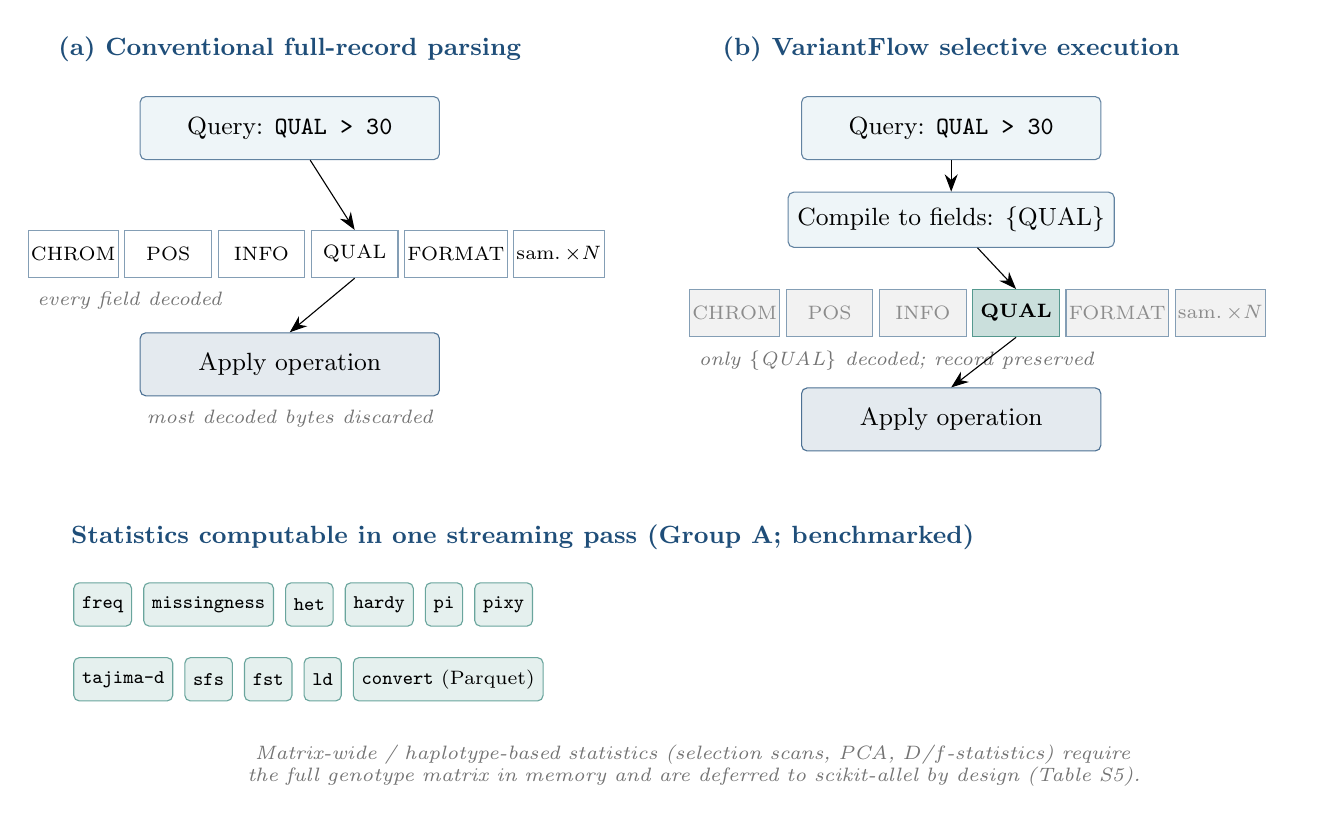
\begin{tikzpicture}[
  font=\small,
  >={Stealth[length=2.2mm]},
  fld/.style={draw=vfblue!55, minimum height=6mm, minimum width=11mm,
              inner sep=1pt, font=\scriptsize, align=center},
  used/.style={fld, fill=vfteal!25, draw=vfteal!80, font=\scriptsize\bfseries},
  skip/.style={fld, fill=black!5, text=black!45},
  stage/.style={draw=vfblue!70, fill=vflight, rounded corners=2pt,
                minimum width=38mm, minimum height=8mm, align=center},
  op/.style={draw=vfblue!80, fill=vfblue!12, rounded corners=2pt,
             minimum width=38mm, minimum height=8mm, align=center},
  hdr/.style={font=\bfseries\small, text=vfblue},
  note/.style={font=\scriptsize\itshape, text=black!55, align=center},
]

% ===== column headers =====
\node[hdr] (hA) at (0,0)   {(a) Conventional full-record parsing};
\node[hdr] (hB) at (8.4,0) {(b) VariantFlow selective execution};

% ===== (a) conventional =====
\node[stage] (aq) at (0,-1.0) {Query: \texttt{QUAL > 30}};
% field strip, decode everything
\node[fld] (a1) at (-2.75,-2.6) {CHROM};
\node[fld,right=0.7mm of a1] (a2) {POS};
\node[fld,right=0.7mm of a2] (a3) {INFO};
\node[fld,right=0.7mm of a3] (a4) {QUAL};
\node[fld,right=0.7mm of a4] (a5) {FORMAT};
\node[fld,right=0.7mm of a5] (a6) {sam.\,$\times N$};
\node[note,below=0.5mm of a1.south west,anchor=north west] (an) {every field decoded};
\node[op] (aop) at (0,-4.0) {Apply operation};
\node[note,below=0.5mm of aop] {most decoded bytes discarded};
\draw[->] (aq) -- (a4.north);
\draw[->] (a4.south) -- (aop.north);

% ===== (b) selective =====
\node[stage] (bq) at (8.4,-1.0) {Query: \texttt{QUAL > 30}};
\node[stage,below=4mm of bq,minimum height=7mm] (bc) {Compile to fields: \{QUAL\}};
\node[skip] (b1) at (5.65,-3.35) {CHROM};
\node[skip,right=0.7mm of b1] (b2) {POS};
\node[skip,right=0.7mm of b2] (b3) {INFO};
\node[used,right=0.7mm of b3] (b4) {QUAL};
\node[skip,right=0.7mm of b4] (b5) {FORMAT};
\node[skip,right=0.7mm of b5] (b6) {sam.\,$\times N$};
\node[note,below=0.5mm of b1.south west,anchor=north west] {only \{QUAL\} decoded; record preserved};
\node[op] (bop) at (8.4,-4.7) {Apply operation};
\draw[->] (bq) -- (bc);
\draw[->] (bc) -- (b4.north);
\draw[->] (b4.south) -- (bop.north);

% ===== statistics band =====
\node[hdr,anchor=west] at (-2.9,-6.2)
  {Statistics computable in one streaming pass (Group A; benchmarked)};
\begin{scope}[chip/.style={draw=vfteal!70, fill=vfteal!12, rounded corners=2pt,
      font=\scriptsize, minimum height=5.5mm, inner sep=3pt, anchor=west}]
  % row 1
  \node[chip] (s1) at (-2.75,-7.05) {\texttt{freq}};
  \node[chip,right=1.4mm of s1] (s2) {\texttt{missingness}};
  \node[chip,right=1.4mm of s2] (s3) {\texttt{het}};
  \node[chip,right=1.4mm of s3] (s4) {\texttt{hardy}};
  \node[chip,right=1.4mm of s4] (s5) {\texttt{pi}};
  \node[chip,right=1.4mm of s5] (s6) {\texttt{pixy}};
  % row 2
  \node[chip] (s7) at (-2.75,-8.0) {\texttt{tajima-d}};
  \node[chip,right=1.4mm of s7] (s8) {\texttt{sfs}};
  \node[chip,right=1.4mm of s8] (s9) {\texttt{fst}};
  \node[chip,right=1.4mm of s9] (s10) {\texttt{ld}};
  \node[chip,right=1.4mm of s10] (s11) {\texttt{convert} (Parquet)};
\end{scope}
\node[note,anchor=west,text width=15.5cm] at (-2.75,-9.1)
  {Matrix-wide / haplotype-based statistics (selection scans, PCA,
   $D$/$f$-statistics) require the full genotype matrix in memory and are
   deferred to scikit-allel by design (Table~S5).};

\end{tikzpicture}

\end{center}

\clearpage
\begin{center}\textbf{Figure 2}\end{center}
\vspace{0.5em}
\begin{center}
% Figure: VariantFlow command tree (left to right: root -> group -> command + description).
% Requires: \usepackage{tikz}; \usetikzlibrary{arrows.meta,positioning,calc};
% colors vfblue, vfteal, vflight.
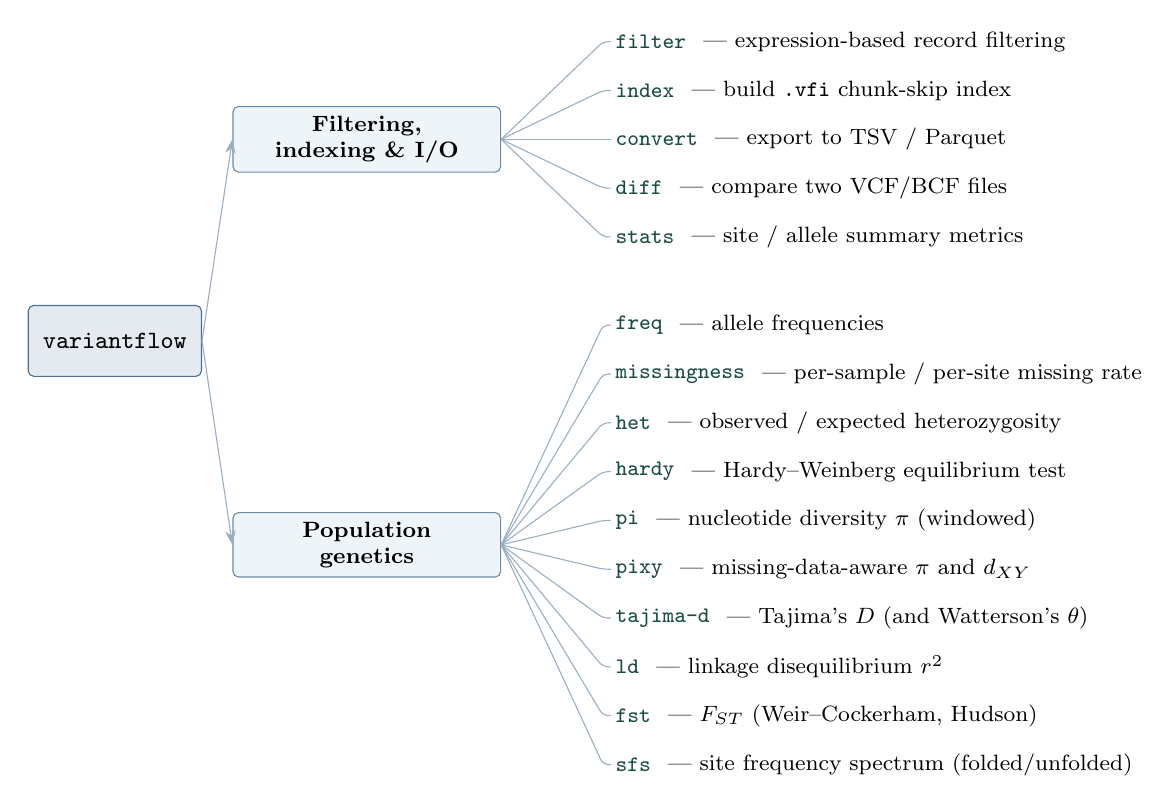
\begin{tikzpicture}[
  font=\small,
  >={Stealth[length=1.8mm]},
  root/.style={draw=vfblue!80, fill=vfblue!12, rounded corners=2pt,
               minimum width=22mm, minimum height=9mm, align=center, font=\ttfamily\small},
  grp/.style={draw=vfblue!65, fill=vflight, rounded corners=2pt,
              minimum width=34mm, minimum height=8mm, align=center, font=\bfseries\footnotesize},
  leaf/.style={anchor=west, font=\footnotesize, inner sep=1.5pt},
  edge/.style={draw=vfblue!45, rounded corners=2pt},
]

\def\lx{6.0}   % leaf x (left anchor)
\newcommand{\leafnode}[3]{\node[leaf] (#1) at (\lx,#2)
  {\textcolor{vfteal!60!black}{\texttt{\textbf{#3}}}};}

% ---- Group A leaves (Filtering, indexing & I/O) ----
\leafnode{filter}{0.0}{filter} \node[leaf,right=1mm of filter] {--- expression-based record filtering};
\leafnode{index}{-0.62}{index} \node[leaf,right=1mm of index] {--- build \texttt{.vfi} chunk-skip index};
\leafnode{convert}{-1.24}{convert} \node[leaf,right=1mm of convert] {--- export to TSV / Parquet};
\leafnode{diff}{-1.86}{diff} \node[leaf,right=1mm of diff] {--- compare two VCF/BCF files};
\leafnode{stats}{-2.48}{stats} \node[leaf,right=1mm of stats] {--- site / allele summary metrics};

% ---- Group B leaves (Population genetics) ----
\leafnode{freq}{-3.6}{freq} \node[leaf,right=1mm of freq] {--- allele frequencies};
\leafnode{miss}{-4.22}{missingness} \node[leaf,right=1mm of miss] {--- per-sample / per-site missing rate};
\leafnode{het}{-4.84}{het} \node[leaf,right=1mm of het] {--- observed / expected heterozygosity};
\leafnode{hardy}{-5.46}{hardy} \node[leaf,right=1mm of hardy] {--- Hardy--Weinberg equilibrium test};
\leafnode{pi}{-6.08}{pi} \node[leaf,right=1mm of pi] {--- nucleotide diversity $\pi$ (windowed)};
\leafnode{pixy}{-6.70}{pixy} \node[leaf,right=1mm of pixy] {--- missing-data-aware $\pi$ and $d_{XY}$};
\leafnode{taj}{-7.32}{tajima-d} \node[leaf,right=1mm of taj] {--- Tajima's $D$ (and Watterson's $\theta$)};
\leafnode{ld}{-7.94}{ld} \node[leaf,right=1mm of ld] {--- linkage disequilibrium $r^{2}$};
\leafnode{fst}{-8.56}{fst} \node[leaf,right=1mm of fst] {--- $F_{ST}$ (Weir--Cockerham, Hudson)};
\leafnode{sfs}{-9.18}{sfs} \node[leaf,right=1mm of sfs] {--- site frequency spectrum (folded/unfolded)};

% ---- group nodes ----
\node[grp] (gA) at (2.9,-1.24) {Filtering,\\indexing \& I/O};
\node[grp] (gB) at (2.9,-6.39) {Population\\genetics};

% ---- root ----
\node[root] (root) at (-0.3,-3.8) {variantflow};

% ---- edges root -> groups ----
\draw[edge,->] (root.east) -- (gA.west);
\draw[edge,->] (root.east) -- (gB.west);

% ---- edges group A -> leaves ----
\foreach \l in {filter,index,convert,diff,stats}{
  \draw[edge] (gA.east) -- ($(\l.west)+(-1mm,0)$) -- (\l.west);
}
% ---- edges group B -> leaves ----
\foreach \l in {freq,miss,het,hardy,pi,pixy,taj,ld,fst,sfs}{
  \draw[edge] (gB.east) -- ($(\l.west)+(-1mm,0)$) -- (\l.west);
}

\end{tikzpicture}

\end{center}

\end{document}
